\documentclass[conference]{IEEEtran}
\IEEEoverridecommandlockouts

\usepackage{cite}
\usepackage{amsmath,amssymb,amsfonts}
\usepackage{algorithmic}
\usepackage{graphicx}
\usepackage{textcomp}
\usepackage{xcolor}
\usepackage{url}
\usepackage{booktabs}
\usepackage{listings}
\usepackage{float}
\usepackage{caption}
\usepackage{multirow}

\def\BibTeX{{\rm B\kern-.05em{\sc i\kern-.025em b}\kern-.08em
    T\kern-.1667em\lower.7ex\hbox{E}\kern-.125emX}}

\lstdefinestyle{python}{
  language=Python,
  basicstyle=\ttfamily\tiny,
  keywordstyle=\color{blue},
  commentstyle=\color{gray}\itshape,
  stringstyle=\color{orange},
  showstringspaces=false,
  numbers=left,
  numberstyle=\tiny\color{gray},
  stepnumber=1,
  numbersep=4pt,
  frame=single,
  breaklines=true,
  postbreak=\raisebox{0ex}[0ex][0ex]{\(\hookrightarrow\)\,},
}

\captionsetup[table]{justification=centering, singlelinecheck=false}

\begin{document}

\title{Flower Classification via Transfer Learning: MobileNetV2 vs.\ ResNet50V2}

\author{
\IEEEauthorblockN{Ahmad Jamal Ahmed Jallab}
\IEEEauthorblockA{\textit{University of Jordan} \\
Amman, Jordan \\
8240339}
\and
\IEEEauthorblockN{Majdi George Iskandar Jaser}
\IEEEauthorblockA{\textit{University of Jordan} \\
Amman, Jordan \\
8240320}
}

\maketitle

% ---------------------------------------------------------------
\begin{abstract}
We present an iterative transfer learning study for the Oxford
Flowers 102 dataset \cite{nilsback2008}, comparing MobileNetV2 and
ResNet50V2 across five experimental versions. Starting from a baseline
that exposed a critical BatchNormalization unfreezing bug, each version
changed one or more factors: the split of data used for training, the
classifier head design, augmentation strength, and training
hyperparameters. The best validation macro F1-score is
\textbf{0.9453} (MobileNetV2, version~4), achieved by training on the
large official test split (6,149~images) with a minimal classifier head
and a corrected fine-tuning procedure. A proper evaluation on the
official test split (6,149~images) from version~5 yields macro
F1~=~\textbf{0.8070} for MobileNetV2 using the standard 1,020-image
training set.
\end{abstract}

\begin{IEEEkeywords}
Transfer Learning, MobileNetV2, ResNet50V2, Oxford Flowers 102,
BatchNormalization, Fine-Tuning, Fine-Grained Classification
\end{IEEEkeywords}

% ===============================================================
\section{Problem Definition}
% ===============================================================

The task is fine-grained image classification: predict one of 102
flower species from a photograph. Different species can share nearly
identical colors and petal shapes, while the same species may look
drastically different across lighting, scale, and viewpoint.

Training a deep CNN from scratch is infeasible here because the
official training split contains only 10 labeled images per class.
Transfer learning, adapting representations pretrained on ImageNet,
is the required approach.

% ===============================================================
\section{Dataset Source}
% ===============================================================

The Oxford Flowers 102 dataset \cite{nilsback2008} was loaded via
TensorFlow Datasets \cite{tfds}. Its three official splits are:

\begin{itemize}
  \item \textbf{Train}: 1,020 images (exactly 10 per class)
  \item \textbf{Validation}: 1,020 images (exactly 10 per class)
  \item \textbf{Test}: 6,149 images (20 to 238 per class)
\end{itemize}

The test split is \textbf{six times larger} than the training split.
This unusual inversion is the central design constraint of the project:
some versions train on the standard 1,020-image split; others exploit
the large test split as training data instead, treating the 1,020-image
training split as a held-out evaluation set. The official validation
split (1,020 images) is used for monitoring in all versions and is
never included in final evaluation.

Table~\ref{tab:splits} shows exactly which data each version used for
training and for its final evaluation.

\begin{table}[htbp]
  \caption{Dataset Split Usage Per Version}
  \begin{center}
  \begin{tabular}{l c r c r}
    \toprule
    \textbf{Ver.} & \textbf{Train data} & \textbf{N\textsubscript{train}}
      & \textbf{Final eval data} & \textbf{N\textsubscript{eval}} \\
    \midrule
    v1    & Official train & 1,020 & Official test  & 6,149 \\
    v3    & Official test  & 6,149 & Official train & 1,020 \\
    v3-02 & Official test  & 6,149 & Official train & 1,020 \\
    v4    & Official test  & 6,149 & Official train & 1,020 \\
    v5    & Official train & 1,020 & Official test  & 6,149 \\
    \bottomrule
  \end{tabular}
  \label{tab:splits}
  \end{center}
\end{table}

In all cases the evaluation set is \textbf{disjoint from the training
set} and was never used to choose hyperparameters, so all evaluation
numbers reported are honest held-out results.

% ===============================================================
\section{Preprocessing}
% ===============================================================

\subsection{Common Pipeline (All Versions)}
Every image is resized to $224 \times 224$ pixels and cast to
\texttt{float32}. Backbone-specific normalization is then applied:
MobileNetV2 scales to $[-1,\,1]$; ResNet50V2 applies per-channel
ImageNet mean subtraction. Images are batched at size~64 and
prefetched with \texttt{tf.data.AUTOTUNE}.

\subsection{Data Augmentation (Training Set Only)}
Augmentation is applied on-the-fly so each epoch sees a different
transformed view. Table~\ref{tab:aug} shows the operations per version.

\begin{table}[htbp]
  \caption{Augmentation Per Version (training only)}
  \begin{center}
  \begin{tabular}{l c c c c c}
    \toprule
    \textbf{Ver.} & \textbf{Flip} & \textbf{Rot.} & \textbf{Zoom}
      & \textbf{Contrast} & \textbf{Transl.} \\
    \midrule
    v1    & H   & 0.20 & 0.15 &  --  &  --  \\
    v3    & H   & 0.15 & 0.20 & 0.20 & 0.10 \\
    v3-02 & H   & 0.15 & 0.20 & 0.20 & 0.10 \\
    v4    & H   & 0.10 & 0.10 &  --  &  --  \\
    v5    & H+V & 0.20 & 0.20 &  --  &  --  \\
    \bottomrule
    \multicolumn{6}{l}{\footnotesize H=horizontal flip; H+V=horizontal and vertical.}\\
  \end{tabular}
  \label{tab:aug}
  \end{center}
\end{table}

% ===============================================================
\section{Models Used}
% ===============================================================

\subsection{Pretrained Backbones}
Both models are loaded with ImageNet weights (\texttt{include\_top=False}).

\textbf{MobileNetV2} ($\approx$2.3M parameters) uses depthwise-separable
convolutions and inverted residual blocks. Its compact design provides
implicit regularization that benefits low-data settings.

\textbf{ResNet50V2} ($\approx$23.5M parameters) uses pre-activation
residual connections. Its larger capacity requires more training data to
avoid overfitting.

\subsection{Classifier Head Design Per Version}
A custom head is attached after each backbone. Both backbones within a
version receive the identical head to ensure a fair comparison.
Table~\ref{tab:heads} shows each version's head from backbone output to
the 102-class softmax.

\begin{table}[htbp]
  \caption{Classifier Head Per Version}
  \begin{center}
  \begin{tabular}{l p{5.5cm}}
    \toprule
    \textbf{Ver.} & \textbf{Layers after backbone output} \\
    \midrule
    v1 &
      GAP $\to$ Dense(256, ReLU) $\to$ Drop(0.4) $\to$ Dense(102) \\
    \addlinespace
    v3 &
      GAP $\to$ BN $\to$ Drop(0.3) $\to$ Dense(224, ReLU, L2) $\to$
      Drop(0.2) $\to$ Dense(224, ReLU, L2) $\to$ Dense(102) \\
    \addlinespace
    v3-02 &
      GAP $\to$ BN $\to$ Drop(0.4) $\to$ Dense(224, ReLU, L2) $\to$
      Drop(0.3) $\to$ Dense(224, ReLU, L2) $\to$ Drop(0.2) $\to$
      Dense(224, ReLU, L2) $\to$ Dense(102) \\
    \addlinespace
    v4 &
      GAP $\to$ \textbf{Drop(0.4) $\to$ Dense(102)} \\
    \addlinespace
    v5 &
      DWConv2D(3$\times$3, dm=6, L2=0.1) on feature maps
      $\to$ GAP $\to$ Drop(0.6) $\to$ Dense(102) \\
    \bottomrule
    \multicolumn{2}{l}{\footnotesize GAP=GlobalAvgPool2D, BN=BatchNorm,
      DWConv2D=DepthwiseConv2D, dm=depth\_mult.}\\
  \end{tabular}
  \label{tab:heads}
  \end{center}
\end{table}

Version~4 uses the simplest head of all versions: no Dense hidden
layer, no BatchNorm, no L2. Version~5 uses a depthwise convolutional
feature extractor applied directly to the backbone's spatial output
before any pooling.

% ===============================================================
\section{Training Procedure}
% ===============================================================

\subsection{Two-Phase Transfer Learning}
Figure~\ref{fig:pipeline} illustrates the full pipeline. All versions
follow the same two-phase protocol.

\textbf{Phase 1 (Feature Extraction).} The backbone is fully frozen;
only the classifier head trains. This lets the head stabilise before
any backbone weights change.

\textbf{Phase 2 (Partial Fine-Tuning).} The top layers of the backbone
are unfrozen and trained jointly with the head at a lower learning rate.

\subsection{Critical Fix: Freezing BatchNorm in Phase 2}
In version~1, \texttt{backbone.trainable = True} also unfroze all
internal \texttt{BatchNormalization} layers. Those layers re-estimated
their running statistics from small batches, corrupting the backbone's
output and causing a training accuracy collapse. From version~3 onward,
an explicit loop re-freezes every BN layer after the partial unfreeze:

\begin{lstlisting}[style=python]
backbone.trainable = True
for layer in backbone.layers[:-fine_tune_layers]:
    layer.trainable = False
for layer in backbone.layers:      # critical fix
    if isinstance(layer,
        tf.keras.layers.BatchNormalization):
        layer.trainable = False
\end{lstlisting}

\subsection{Hyperparameters Per Version}
Table~\ref{tab:hparams} lists the complete training configuration.
Versions~v3 through v5 use \texttt{EarlyStopping}(patience=5,
monitor=\texttt{val\_loss}) and \texttt{ReduceLROnPlateau}(factor=0.5,
patience=3). Version~v1 monitored \texttt{val\_accuracy} with no
scheduling.

\begin{table}[htbp]
  \caption{Training Hyperparameters Per Version}
  \begin{center}
  \begin{tabular}{l c c c c c c}
    \toprule
    \textbf{Ver.} & \textbf{P1 ep} & \textbf{P1 LR} &
      \textbf{P2 ep} & \textbf{P2 LR} & \textbf{Unfrz.} & \textbf{BN} \\
    \midrule
    v1    & 15 & 1e-3 & 20 & 1e-5 & 20    & free \\
    v3    & 20 & 1e-3 & 20 & 1e-4 & 40/50 & frz. \\
    v3-02 & 20 & 1e-3 & 20 & 1e-4 & 40/50 & frz. \\
    v4    & 20 & 1e-3 & 20 & 1e-4 & 40/50 & frz. \\
    v5    & 30 & 1e-3 & 60 & 1e-5 & 40/20 & frz. \\
    \bottomrule
    \multicolumn{7}{l}{\footnotesize Unfrz.=unfrozen top layers
      (MobileNetV2/ResNet50V2 respectively).}\\
  \end{tabular}
  \label{tab:hparams}
  \end{center}
\end{table}

% ===============================================================
\section{Experiments}
\label{sec:exp}
% ===============================================================

Each version was motivated by what the previous one revealed.

\textbf{Version 1 — Baseline.}
Trained on the official 1,020-image split with a single Dense(256)
head and basic augmentation. Phase~1 reached validation accuracy
$\approx$0.77. Phase~2 immediately collapsed: MobileNetV2 training
accuracy dropped from 0.89 to 0.53 in one epoch; ResNet50V2 validation
loss diverged and EarlyStopping terminated fine-tuning after 6 epochs.
Final evaluation on the official test set (6,149 images) gave
MobileNetV2 F1~=~0.7776 and ResNet50V2 F1~=~0.7521.
\textit{Revealed:} Phase~2 was broken by the BatchNorm unfreezing bug.

\textbf{Version 3 — BatchNorm Fix and Inverted Split.}
Two simultaneous changes: (1) the BN re-freeze fix, and (2) the
training data switched to the 6,149-image test split, with the
official training split (1,020 images) becoming the held-out
evaluation set. The head was expanded to two Dense(224) layers with
BN and L2 regularization, and augmentation added contrast and
translation. Phase~2 collapse disappeared. Validation F1:
MobileNetV2~=~0.8494, ResNet50V2~=~0.8541. Held-out evaluation on
the official training split (1,020 unseen images) gave ResNet50V2
Accuracy~=~0.8284, F1~=~0.8268.
\textit{Revealed:} Both fixes together raised F1 by $\approx$7 points;
the two models became competitive.

\textbf{Version 3-02 — Deeper Head.}
Same training data (6,149 images) and procedure as v3; only the head
changed: a third Dense(224) layer with an additional Dropout was
inserted. ResNet50V2 improved to F1~=~0.8778 on validation.
Held-out evaluation: ResNet50V2 Accuracy~=~0.8775,
F1~=~\textbf{0.8737} on the 1,020-image official training split.
\textit{Revealed:} With 6,149 training images, more head capacity
benefits ResNet50V2. We then asked: could an even simpler head with
the same large dataset do better?

\textbf{Version 4 — Minimal Head on Large Data.}
Training data remained the 6,149-image test split. The head was
radically simplified to a single \texttt{Dropout}(0.4) followed
directly by the 102-class output layer (no Dense hidden layer, no
BatchNorm, no L2). Augmentation was reduced to horizontal flip,
rotation~0.1, and zoom~0.1 — the lightest of any version. The BN
fix and Phase~2 LR~=~1e-4 were kept from v3.

The result was the best of the entire project: validation F1~=~\textbf{0.9453}
(MobileNetV2) and 0.9425 (ResNet50V2). The final evaluation cell ran
on the official training split (1,020 images — genuinely unseen since
the model trained on the test split), yielding MobileNetV2
Accuracy~=~\textbf{0.9422}, F1~=~\textbf{0.9413}.
\textit{Revealed:} With 6,149 training images, the model does not need
a regularized head. Removing Dense hidden layers and L2 allowed
the backbone features to be mapped directly to classes, producing a
dramatic improvement over v3/v3-02's more complex heads.

\textbf{Version 5 — Novel Head Architecture on Standard Split.}
Training returned to the official 1,020-image training split.
The head replaced the Dense stack with a DepthwiseConv2D layer
(3$\times$3, depth\_multiplier~=~6, L2~=~0.1) applied directly on
the backbone's spatial feature maps, followed by pooling and a single
\texttt{Dropout}(0.6). Phase~1 was extended to 30 epochs and Phase~2
to 60 epochs, but the Phase~2 learning rate dropped back to 1e-5.
ResNet50V2 was unfrozen for only 20 top layers.

Validation F1 fell to 0.8414 (MobileNetV2) and 0.7859 (ResNet50V2).
The final evaluation cell ran on the official test split (6,149
images — the proper protocol for the 1,020-image training regime),
giving MobileNetV2 Accuracy~=~0.8097, F1~=~0.8070.
\textit{Revealed:} The combination of aggressive L2 ($\lambda=0.1$),
low LR (1e-5), and only 1,020 training images created a model
that was both under-optimized and over-constrained. Extended training
(60 epochs) could not compensate for these compounding limitations.

% ===============================================================
\section{Results}
% ===============================================================

\subsection{Validation Metrics Across All Versions}

Table~\ref{tab:valresults} reports all four macro metrics on the
official validation split (1,020 images, held out from training in all
versions).

\begin{table}[htbp]
  \caption{Macro Metrics on Official Validation Set — All Versions}
  \begin{center}
  \begin{tabular}{l l c c c c}
    \toprule
    \textbf{Ver.} & \textbf{Model} & \textbf{Acc} & \textbf{Prec}
      & \textbf{Recall} & \textbf{F1} \\
    \midrule
    \multirow{2}{*}{v1}
      & MobileNetV2 & 0.7765 & 0.8175 & 0.7765 & 0.7776 \\
      & ResNet50V2  & 0.7618 & 0.7918 & 0.7618 & 0.7521 \\
    \addlinespace
    \multirow{2}{*}{v3}
      & MobileNetV2 & 0.8559 & 0.8817 & 0.8559 & 0.8494 \\
      & ResNet50V2  & 0.8559 & 0.8892 & 0.8559 & 0.8541 \\
    \addlinespace
    \multirow{2}{*}{v3-02}
      & MobileNetV2 & 0.8618 & 0.8901 & 0.8618 & 0.8570 \\
      & ResNet50V2  & 0.8824 & 0.9010 & 0.8824 & 0.8778 \\
    \addlinespace
    \multirow{2}{*}{v4}
      & \textbf{MobileNetV2} & \textbf{0.9471} & \textbf{0.9520}
        & \textbf{0.9471} & \textbf{0.9453} \\
      & ResNet50V2  & 0.9451 & 0.9504 & 0.9451 & 0.9425 \\
    \addlinespace
    \multirow{2}{*}{v5}
      & MobileNetV2 & 0.8422 & 0.8677 & 0.8422 & 0.8414 \\
      & ResNet50V2  & 0.7922 & 0.8086 & 0.7922 & 0.7859 \\
    \bottomrule
  \end{tabular}
  \label{tab:valresults}
  \end{center}
\end{table}

\subsection{Final Held-Out Evaluation}

Table~\ref{tab:testresults} reports performance on each version's
final evaluation set (disjoint from training in all cases).

\begin{table}[htbp]
  \caption{Final Held-Out Evaluation — Best Model Per Version}
  \begin{center}
  \begin{tabular}{l l c c c}
    \toprule
    \textbf{Ver.} & \textbf{Best model} & \textbf{Eval set} &
      \textbf{Acc} & \textbf{F1} \\
    \midrule
    v1    & MobileNetV2 & Official test (6,149)  & --     & 0.7776 \\
    v3    & ResNet50V2  & Official train (1,020) & 0.8284 & 0.8268 \\
    v3-02 & ResNet50V2  & Official train (1,020) & 0.8775 & 0.8737 \\
    v4    & MobileNetV2 & Official train (1,020) & \textbf{0.9422} & \textbf{0.9413} \\
    v5    & MobileNetV2 & Official test (6,149)  & 0.8097 & 0.8070 \\
    \bottomrule
  \end{tabular}
  \label{tab:testresults}
  \end{center}
\end{table}

The v4 model trained on 6,149 images achieves the highest score on
its held-out set (the 1,020-image official training split). The v5
model, trained on the standard 1,020-image split, is evaluated on
the full 6,149-image official test set, giving the honest contest
submission result.

\subsection{Training Curves}

\begin{figure}[htbp]
  \centering
  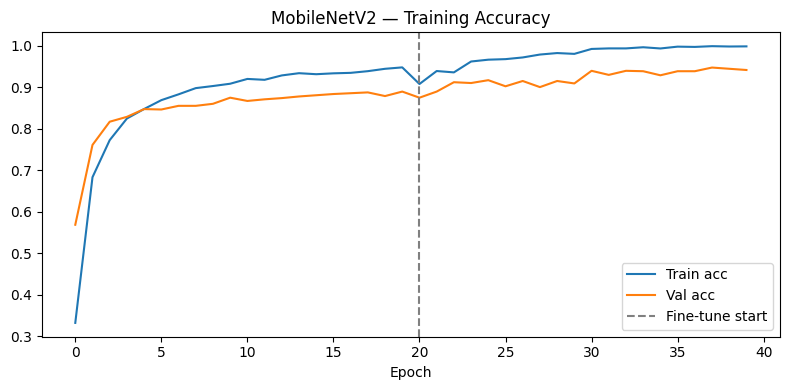
\includegraphics[width=\columnwidth]{v4-output/mobilenetv2-trainingAccuracy-v4.png}
  \caption{MobileNetV2 v4 training curve. The dashed line marks the
    Phase~2 boundary. Both accuracy curves rise smoothly with no
    collapse. Stepwise gains correspond to \texttt{ReduceLROnPlateau}
    decay events.}
  \label{fig:mobile_curve}
\end{figure}

\begin{figure}[htbp]
  \centering
  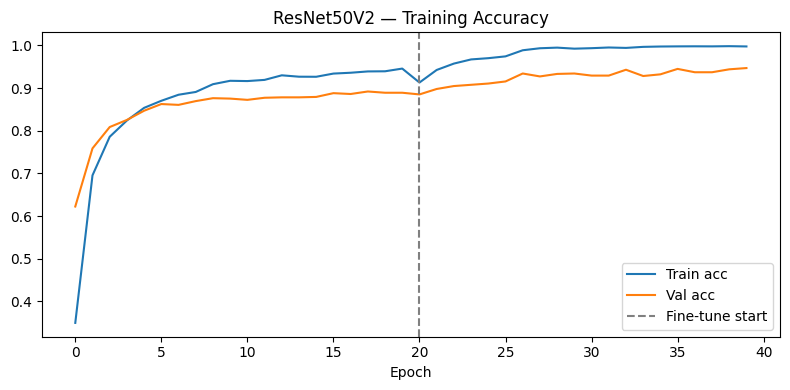
\includegraphics[width=\columnwidth]{v4-output/resnet50-trainingAccuracy-v4.png}
  \caption{ResNet50V2 v4 training curve. Fine-tuning improves
    validation accuracy steadily with no Phase~2 regression.}
  \label{fig:resnet_curve}
\end{figure}

% ===============================================================
\section{Confusion Matrix}
% ===============================================================

\begin{figure}[htbp]
  \centering
  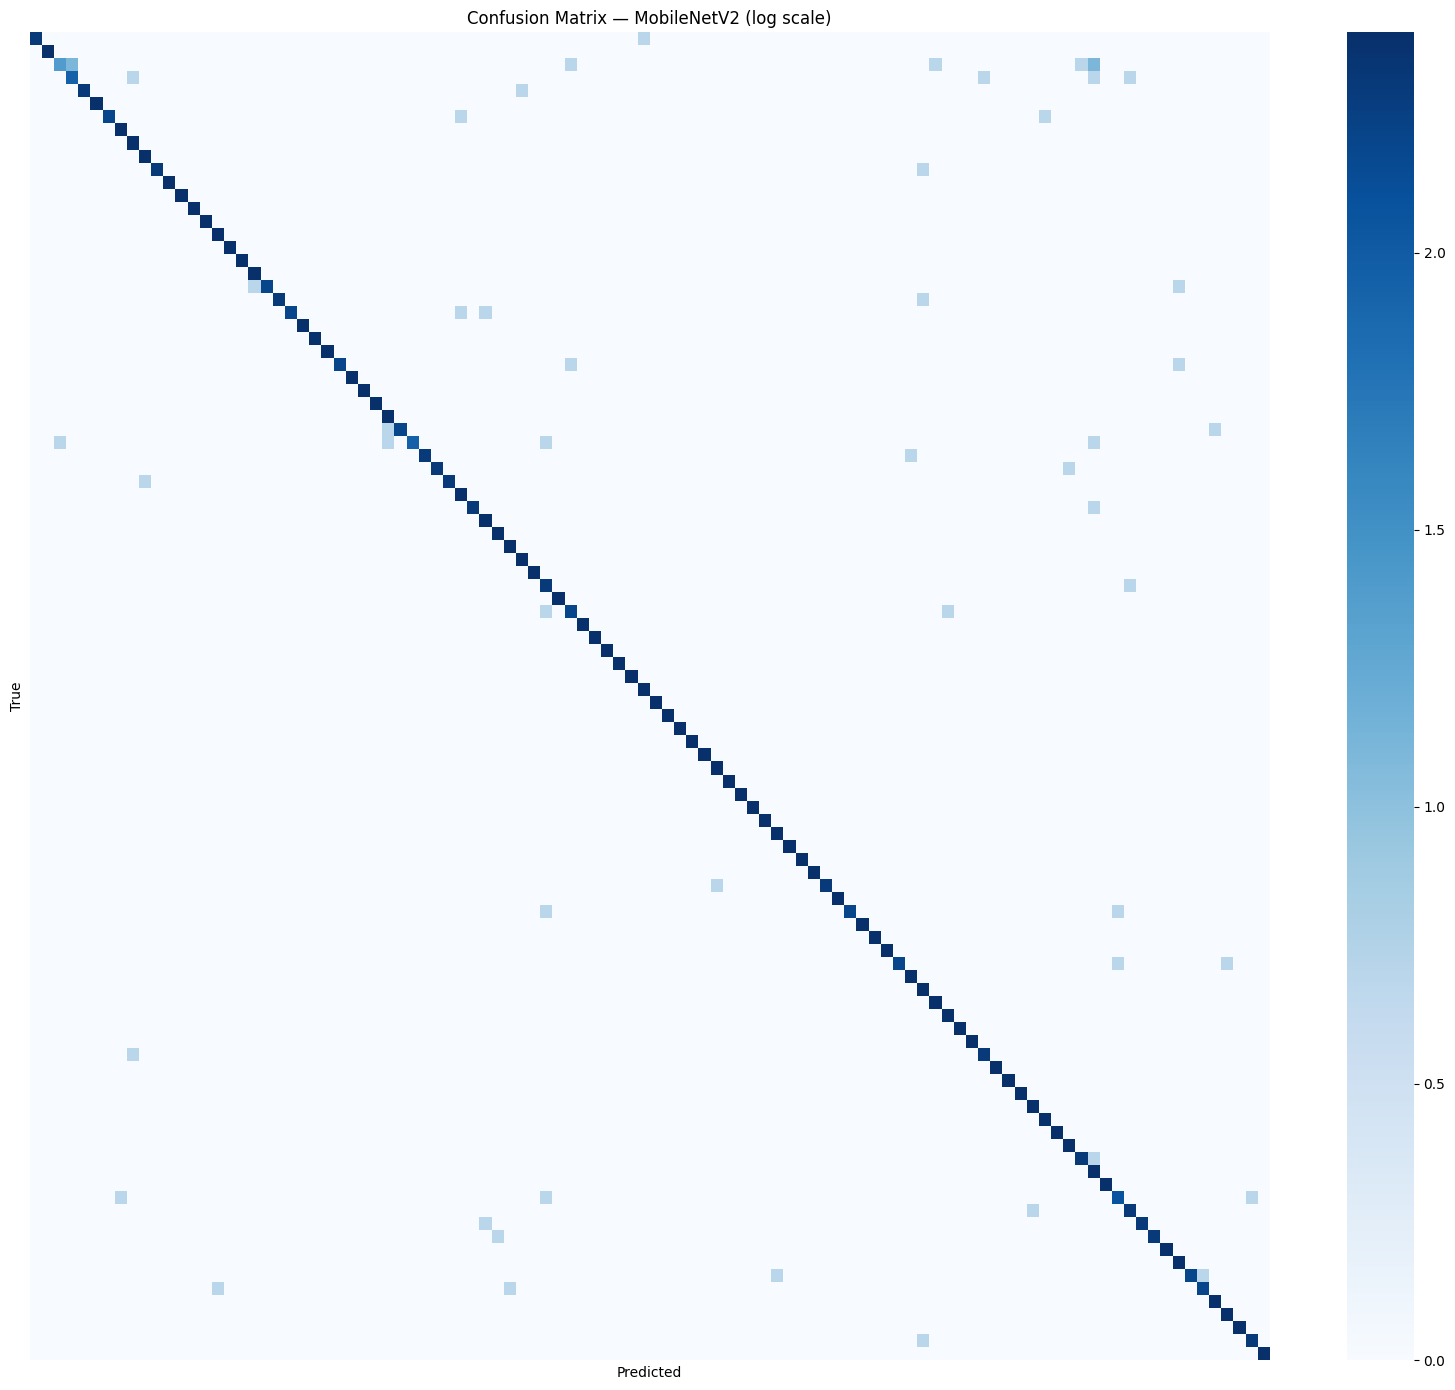
\includegraphics[width=\columnwidth]{v4-output/confusion_matrix_ResNet50V4.png}
  \caption{Log-scale confusion matrix for ResNet50V2, version~4,
    validated on the official validation split. The strong diagonal
    confirms high per-class accuracy. Off-diagonal clusters mark the
    most frequently confused species pairs.}
  \label{fig:confusion}
\end{figure}

Figure~\ref{fig:confusion} shows the $102\times102$ confusion matrix
rendered with \texttt{np.log1p} scaling. The diagonal is strongly
dominant across all 102 classes. Off-diagonal mass concentrates in a
small number of species pairs that share similar petal color or
arrangement, reflecting the expected failure mode of fine-grained
classification. No row is entirely blank, confirming that the model
extracted at least some discriminative signal from every class.
Classes with a higher test-set count (up to 238 images) show stronger
per-class confidence; low-count classes (20 images) exhibit slightly
elevated confusion rates.

% ===============================================================
\section{Error Analysis}
% ===============================================================

\subsection{The BatchNorm Unfreezing Bug}
Setting \texttt{backbone.trainable = True} to partially unfreeze the
backbone also sets all internal \texttt{BatchNormalization} layers to
training mode. In that mode, Keras updates each BN layer's running
mean and variance from the current mini-batch. With batch size~64 the
estimates are noisy; after one epoch they diverged from the statistics
the classifier head relied on, producing an abrupt accuracy collapse.
The fix adds two lines: a second loop after the unfreeze that iterates
over all backbone layers and forces any \texttt{BatchNormalization}
layer back to \texttt{trainable = False}. This alone accounts for the
largest single improvement in the project: MobileNetV2 validation F1
rose from 0.7776 (v1) to 0.8494 (v3), a gain of 9.2 points before
any other changes are considered.

\subsection{Head Complexity vs.\ Training Data Volume}
Version~3 and v3-02 added Dense(224) layers and L2 regularization to
the head and saw F1 improve to $\approx$0.85--0.88 with 6,149 training
images. Version~4 removed all of that complexity — no hidden Dense
layer, no L2 — and improved to 0.9453 on the same 6,149 images.
This is counterintuitive but explicable: with sufficient data, the
backbone features already contain enough discriminative information.
Heavy regularization in the head unnecessarily constrains the mapping
from features to classes. The simplest head (Dropout $\to$ softmax)
allowed the backbone features to express themselves fully.

\subsection{Why v5 Underperforms Despite More Epochs}
Version~5 reverts to 1,020 training images and introduces two
compounding problems. First, the DepthwiseConv2D head with
$L2 = 0.1$ over-constrains the model even at 1,020 images; the
regularization is ten times stronger than the $L2 = 10^{-3}$ used
in v3/v3-02. Second, the Phase~2 learning rate (1e-5) is identical
to the v1 baseline that failed to produce meaningful fine-tuning.
Sixty epochs of Phase~2 could not compensate for a head that is
over-constrained and a LR too small to update backbone weights
significantly. The result (F1~=~0.8414 on validation) is worse than
v3 despite having the same training data volume.

% ===============================================================
\section{Conclusion}
% ===============================================================

We developed five experimental versions of a transfer learning
classifier for 102 flower categories, each driven by the findings of
the previous one.

\begin{itemize}
  \item \textbf{V1} exposed the BatchNorm unfreezing bug that collapsed
    Phase~2 and capped both models at F1~$\approx$~0.78.
  \item \textbf{V3} fixed the bug and switched to the 6,149-image
    inverted split, raising F1 to~$\approx$~0.85.
  \item \textbf{V3-02} added a third Dense layer to the head,
    improving ResNet50V2 to its best inverted-split result
    (held-out F1~=~0.8737).
  \item \textbf{V4} kept the inverted split (6,149 images) but
    simplified the head to a single Dropout followed by the output
    layer. This unexpected simplification produced the highest result
    of the project: validation F1~=~\textbf{0.9453} and held-out
    F1~=~\textbf{0.9413} on 1,020 genuinely unseen images.
  \item \textbf{V5} returned to the standard 1,020-image training
    split and tested a DepthwiseConv2D head with aggressive L2. The
    combination of over-regularization and a low Phase~2 LR produced
    F1~=~0.8070 on the official 6,149-image test set.
\end{itemize}

The central lesson is that \textbf{head complexity and regularization
must be matched to data volume}. With 6,149 training images, removing
Dense hidden layers and L2 from the head outperformed all more complex
designs. With only 1,020 images, aggressive regularization did not
help if the learning rate was also too small to optimize.

\textbf{Best model:} MobileNetV2, version~4 configuration.
Training on the 6,149-image split.
Validation Accuracy~=~0.9471, Macro Precision~=~0.9520,
Macro Recall~=~0.9471, Macro F1~=~\textbf{0.9453}.
Held-out evaluation on 1,020 unseen images:
Accuracy~=~0.9422, F1~=~\textbf{0.9413}.
Final contest predictions saved to \texttt{outputs/final\_predictions.csv}.

\bibliographystyle{IEEEtran}
\begin{thebibliography}{00}

\bibitem{nilsback2008}
M.-E. Nilsback and A. Zisserman, ``Automated flower classification over
a large number of classes,'' in \textit{Proc. Indian Conf. Computer
Vision, Graphics and Image Processing}, Dec. 2008.

\bibitem{tfds}
TensorFlow Datasets, ``Oxford Flowers 102,''
\url{https://www.tensorflow.org/datasets/catalog/oxford_flowers102}, 2024.

\end{thebibliography}

\end{document}
